%% ----------------------------------------------------------------
%% Thesis.tex -- MAIN FILE (the one that you compile with LaTeX)
%% ----------------------------------------------------------------

% Set up the document
\documentclass[a4paper, 11pt, oneside]{Thesis}  % Use the "Thesis" style, based on the ECS Thesis style by Steve Gunn
\graphicspath{Figures/}  % Location of the graphics files (set up for graphics to be in PDF format)

% Include any extra LaTeX packages required
\usepackage[square, numbers, comma, sort&compress]{natbib}  % Use the "Natbib" style for the references in the Bibliography
\usepackage{verbatim}  % Needed for the "comment" environment to make LaTeX comments
\usepackage{vector}  % Allows "\bvec{}" and "\buvec{}" for "blackboard" style bold vectors in maths
\hypersetup{urlcolor=blue, colorlinks=true}  % Colours hyperlinks in blue, but this can be distracting if there are many links.
\usepackage{url}

%% ----------------------------------------------------------------
\begin{document}
\frontmatter      % Begin Roman style (i, ii, iii, iv...) page numbering

% Set up the Title Page
\title  {Flexible Management of Superpages to Improve Performance}
\authors  {\texorpdfstring
            {David Lindenbaum}
            {Author Name}
            }
\addresses  {\groupname\\\deptname\\\univname}  % Do not change this here, instead these must be set in the "Thesis.cls" file, please look through it instead
\date       {\today}
\subject    {}
\keywords   {}

\maketitle
%% ----------------------------------------------------------------

\setstretch{1.3}  % It is better to have smaller font and larger line spacing than the other way round

% Define the page headers using the FancyHdr package and set up for one-sided printing
\fancyhead{}  % Clears all page headers and footers
\rhead{\thepage}  % Sets the right side header to show the page number
\lhead{}  % Clears the left side page header

\pagestyle{fancy}  % Finally, use the "fancy" page style to implement the FancyHdr headers

\clearpage
%% ----------------------------------------------------------------

% The Abstract Page
\addtotoc{Abstract}  % Add the "Abstract" page entry to the Contents
\abstract{
\addtocontents{toc}{\vspace{1em}}  % Add a gap in the Contents, for aesthetics

Superpages are a contiguous set of virtual pages mapped to a contiguous set of physical frames (typically 2MB or 1GB in size). They allow the processor to use a single TLB entry to express the virtual-to-physical mapping of a large range of addresses, thereby reducing overall TLB misses. Unfortunately, superpages reduce the flexibility for the operating system to efficiently manage memory. Techniques like copy-on-write are much more expensive when superpages are in use because the entire superpage must be copied for even a small write.

Our work examines changes to the TLB that make it possible to gain the advantages of superpages without losing the flexibility of standard pages. In particular, we propose a system called ``superpage overlays'' which allows the system to track modifications to superpages at a page granularity. It does this by appending a bit vector to each page table and TLB entry, indicating which segments of the superpage are mapped to an ``overlay'' instead and are translated via a secondary page table hierarchy.

Our system alleviates the downsides of superpages. Overlays can track small changes in superpages to avoid copying the full superpage or breaking it down into standard pages. Rather than doing a copy-on-write, we can create an overlay on write and only copy one page while preserving the original superpage. To evaluate the proposal we use a trap-driven simulation framework that simulates the behavior of the TLB in situ while benchmarks are running.

}

\clearpage  % Abstract ended, start a new page
%% ----------------------------------------------------------------

\setstretch{1.3}  % Reset the line-spacing to 1.3 for body text (if it has changed)
\pagestyle{fancy}  %The page style headers have been "empty" all this time, now use the "fancy" headers as defined before to bring them back


%% ----------------------------------------------------------------
\lhead{\emph{Contents}}  % Set the left side page header to "Contents"
\tableofcontents  % Write out the Table of Contents

%% ----------------------------------------------------------------
\lhead{\emph{List of Figures}}  % Set the left side page header to "List if Figures"
\listoffigures  % Write out the List of Figures

%% ----------------------------------------------------------------
% End of the pre-able, contents and lists of things
% Begin the Dedication page

\setstretch{2}  % Return the line spacing back to 1.3
\lhead{}

\mainmatter	  % Begin normal, numeric (1,2,3...) page numbering
\pagestyle{fancy}  % Return the page headers back to the "fancy" style

% Include the chapters of the thesis, as separate files
% Just uncomment the lines as you write the chapters

% !TEX root = ../Thesis.tex
\chapter{Introduction}

Page-based virtual memory transparently allocates different parts of the physical memory to each process in units of fixed-sized pages, which are 4KB in nearly all modern systems. The translations between virtual and physical addresses are stored in a hierarchy of page tables (4 levels in modern AMD64 systems). Each page table is a list of page table entries (PTEs) that contain a pointer to the next level or the final physical address. Some architectures, including AMD64, support creating superpages (sometimes known as large pages or huge pages) by setting a flag in the page table entry that stops the page table walk before the final level. The resulting superpages are thus 2MB or 1GB in size on AMD64.

The Translation Lookaside Buffer (TLB) caches virtual-to-physical translations so that the memory-management unit (MMU) does not need to walk the page tables for every memory access. The TLB is critical to performance and TLB misses add significant overhead to execution time in many workloads \cite{Barr}. Superpages offer a reduction in TLB misses by allowing larger regions of memory to be represented with one TLB entry. The TLB has separate groups of entries for 2MB, 1GB, and the regular 4KB pages. In addition to reducing TLB misses, superpages make the cost of a TLB miss slightly smaller because the page table walk only has three steps instead of four.

While superpages can increase TLB reach and thus reduce misses, they are less flexible than 4KB pages because they map a larger contiguous region of memory. PTEs include flags that mark various properties of the page, such as whether or not it has a mapping to physical memory, whether it is writeable or read-only, and whether it is accessible to the user or only the kernel. Since these flags apply to the entire region mapped by a PTE, 4KB pages allow much finer-grained management than superpages.

The Linux kernel has a system called Transparent Hugepages (THP) which automatically creates 2MB superpages whenever large blocks of memory are allocated or previously-allocated blocks of memory are found to be alligned to 2MB \cite{THP}. This enables any program to gain the advantages of superpages without being written with them in mind. To maintain transparency to userspace, THP are automatically split whenever an operation is done that would change the flags of one of the pages it contains.

\section{Prior Work}

Other groups have proposed ways to gain most of the benefits of superpages without the downsides. The GLUE \cite{Pham} and SpecTLB \cite{Barr} systems both use speculative TLB entries to map 2MB regions of virtual addresses that are mostly aligned. GLUE is software-transparent, which means that the TLB automatically creates speculative entries and the operating system does not need to be changed to support it. SpecTLB, on the other hand, requires minor operating system changes to explicitly mark speculative superpages. Since both of these systems are speculative in nature, there are some major downsides. A speculation failure will incur a significant overhead to roll back everything the processor did with the incorrect translation, and the infrastructure required to do so complicates the entire memory management system. However, they do show significant reductions in TLB misses as a result of improved superpage utilization.

\section{Superpage Overlays}

Our proposed solution to the downsides of superpages is to use a system called ``overlays'' to allow more flexible management of superpages and achieve the best of both worlds. In addition to the existing mapping from a virtual superpage to contiguous physical memory, each 4KB page with the superpage can optionally map to an overlay, which overrides the virtual-to-physical mapping for that page (see figure \ref{fig:basic}). The set of pages within a superpage that map to overlays is defined by the overlay bit vector (OBitVector). With this system, copy-on-write can be replaced with overlay-on-write. Instead of copying the entire superpage, an overlay is created for one 4KB region in the address space of the writing process. Thus, only 4KB needs to be copied and the rest of the superpage still exists for both processes, providing the usual memory utilization and TLB reach improvements.

The superpage overlay system presented here is based on page overlays from another recent work \cite{Seshadri}. That framework used overlays the size of a cache line for very fine-grained management of regular pages. Superpage overlays are simpler in that they can simply extend the existing page table system and thus require less significant changes to the MMU.

This project makes three main contributions. First, we describe the superpage overlay framework and show how it would be implemented. Second, we describe the trap-driven simulation infrastructure that can be used to test the effectiveness of superpage overlays without using the modified hardware that the framework requires. Third, we show the benefits of superpage overlays for some example applications.

\begin{figure}
    \centering
    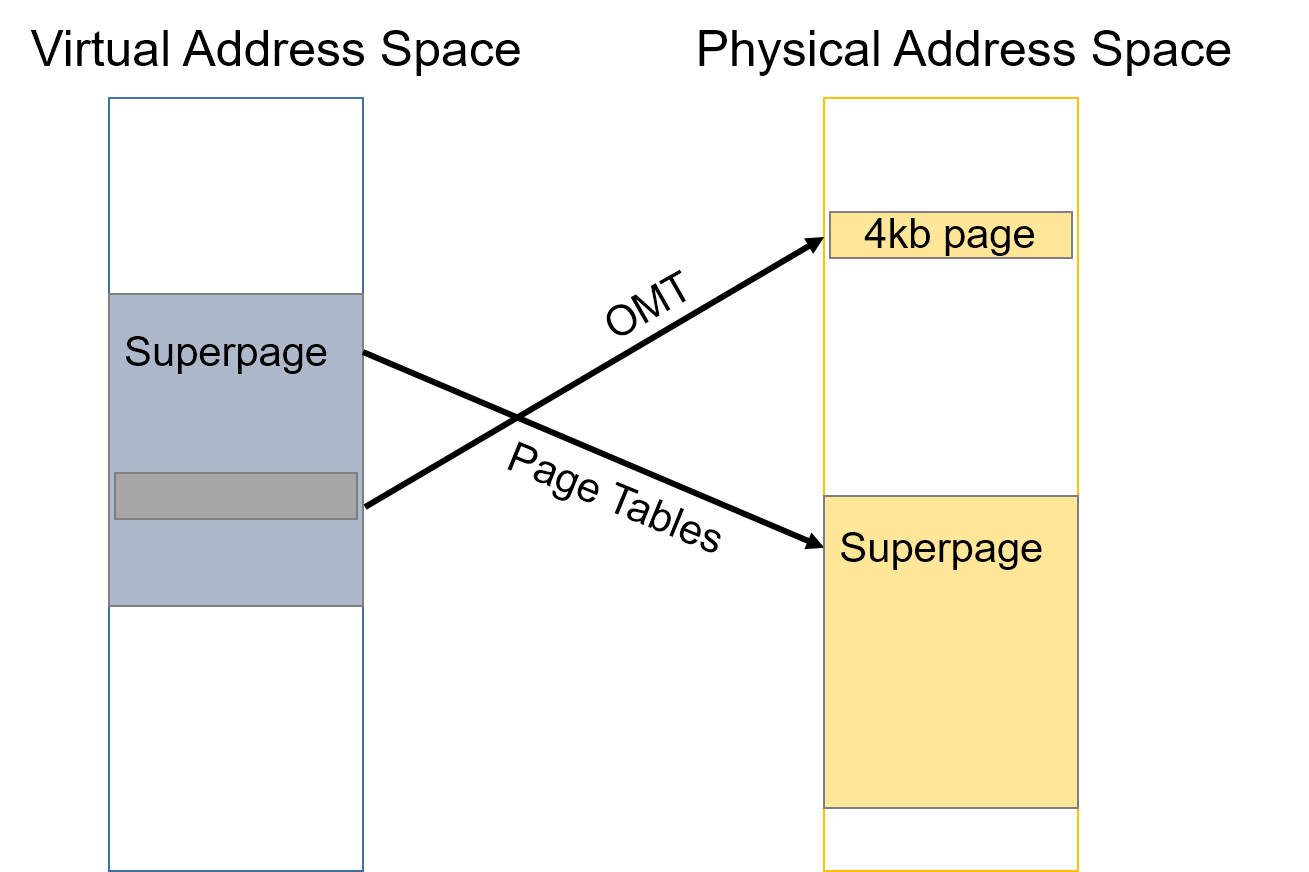
\includegraphics[width=3in]{Figures/Picture1}
    \caption{A basic diagram of the virtual-to-physical mappings for a superpage with overlay}
    \label{fig:basic}
\end{figure}
 % Introduction

\chapter{Superpage Overlay Design}

To identify which parts of a superpage are mapped to an overlay, the OBitVector is appended to the TLB entries for superpages. On a TLB hit for a 2MB superpage, the lower-order bits of the address are used to check the corresponding index in the OBitVector. If it is 0, the translation is returned as normal. If it is 1, the 4KB TLB is checked instead. On TLB miss is this situation, the memory controller can either walk the page tables as normal or proceed directly to the Overlay Mapping Table (OMT), since there is guaranteed to be an overlay for this address.

The OMT is simply a secondary page table hierarchy, which maps addresses that have overlays to the physical location of the overlay. The OBitVector for an address not present at the 2MB level of the OMT is 0. Otherwise it simply consists of the present bits of the next level page table. On a TLB miss of any kind, the memory controller walks the regular page table as normal. Concurrently, it walks the OMT and overrides the mapping if the address is present there. Both translations and the OBitVector are then cached in the TLB.

\section{Performance Impact}
In the case of a hit in the 2MB TLB, performance will be only very slightly impacted by the requirement of testing one additional bit. Hits in the 4KB TLB are completely unchanged. Thus, in the common case superpage overlays do not hurt performance, and the increased TLB reach offered by better superpage utilization makes that case even more common.

The page table walk is complicated by the requirement of walking an additional page table hierarchy, but the two operations can be done concurrently and the OMT walk will quickly stop in the common case where there are no overlays. The largest performance impact is likely the increased cache pressure, since there are simply more page tables to cache.

\section{Possible Variants}
The above outlines the simplest version of the superpage overlay framework, which just adds OBitVectors to the 2MB TLB and an additional page table hierarchy that is no different from the existing one. There are three variants that could improve the performance of the modified page table walk at the cost of greater page table and memory controller complexity.

The simplest one is to store the OBitVector directly in the 2MB level of the OMT rather than building it by examining the present bits of the next level table. This reduces the number of entries that can be stored in a single-page OMT table, since the OBitVector must be stored for each entry. It likely yields a significant performance improvement to the OMT walk, especially since it puts the OBitVector on a single cache line.

The second variant is storing the OBitVector in the regular page table instead of the OMT, which allows the OMT walk to not occur at all in the common case. Altering the structure of the existing page table is a much greater cost than altering the newly proposed OMT, however.

Finally, both the OBitVector and the overlay mappings could be stored directly in the 2MB level of the regular page table. This eliminates the OMT altogether, and the page table walk just stops at the 2MB level like a regular superpage or continues to the 4KB level like a regular page depending on the OBitVector test. That would result in almost no performance impact on the page table walk, but increasing the size of page table entries by that much would likely hurt performance in other areas too greatly.

All three of these variants could be tuned by using a smaller OBitVector where each bit applies to multiple 4KB pages. This reduces the flexibility improvements because superpages can only be managed at the granularity that the OBitVector allows, but it reduces the impact on the size of page table entries.

The second variant was the initial design for superpage overlays, with the third being considered as well. After considering the impact those would have on the whole page table structure, I developed the basic approach and first variant as simpler options.

\section{Hardware Cost}
Enabling superpage overlays requires changing the hardware in the TLB and the MMU, but the changes are relatively simple. A bit vector must be added to each 2MB TLB entry, and the logic for a TLB hit changed to test the bit vector and defer to the 4KB TLB for overlays. The MMU must be modified to walk the OMT along with the regular page tables, but the logic is mostly the same so the cost should be relatively low.

\section{Application: Overlay-on-Write}
The main application of superpage overlays presented is overlay-on-write. This changes the copy-on-write policy for superpages to avoid copying the entire superpage. In existing systems, when a process is forked the new process maps to the same physical pages as the parent, and all writable pages are marked read-only for copy-on-write. When a write is made to a superpage marked for copy-on-write, the whole page is copied and the page table for the writing process is updated to point to the new superpage. With overlay-on-write, only the 4KB section of the superpage that is written is copied, and that new page is added to the OMT for the writing process. Figure \ref{fig:oow} visualizes the difference. As a result, much less data is copied if the processes only change a small portion of their writable pages.

This change occurs in the OS, since the OMT can be managed in the same way as the existing page tables and the OS is already responsible for implementing copy-on-write. It reduces data duplication in memory and increases performance by allowing two processes that share most of their data to point to the same physical superpage even when there are some differences. Once a certain portion of the superpage is mapped to overlays, the OS should switch to regular mappings to eliminate the overhead of having too many overlays. This can be done by either copying the superpage and removing the overlays, or removing the superpage and turning the overlays into regular 4KB page mappings. The first option preserves the superpage but requires more data to be copied, while the second option does not copy any data but loses the advantages of keeping it in superpages.
\begin{figure}
    \centering
    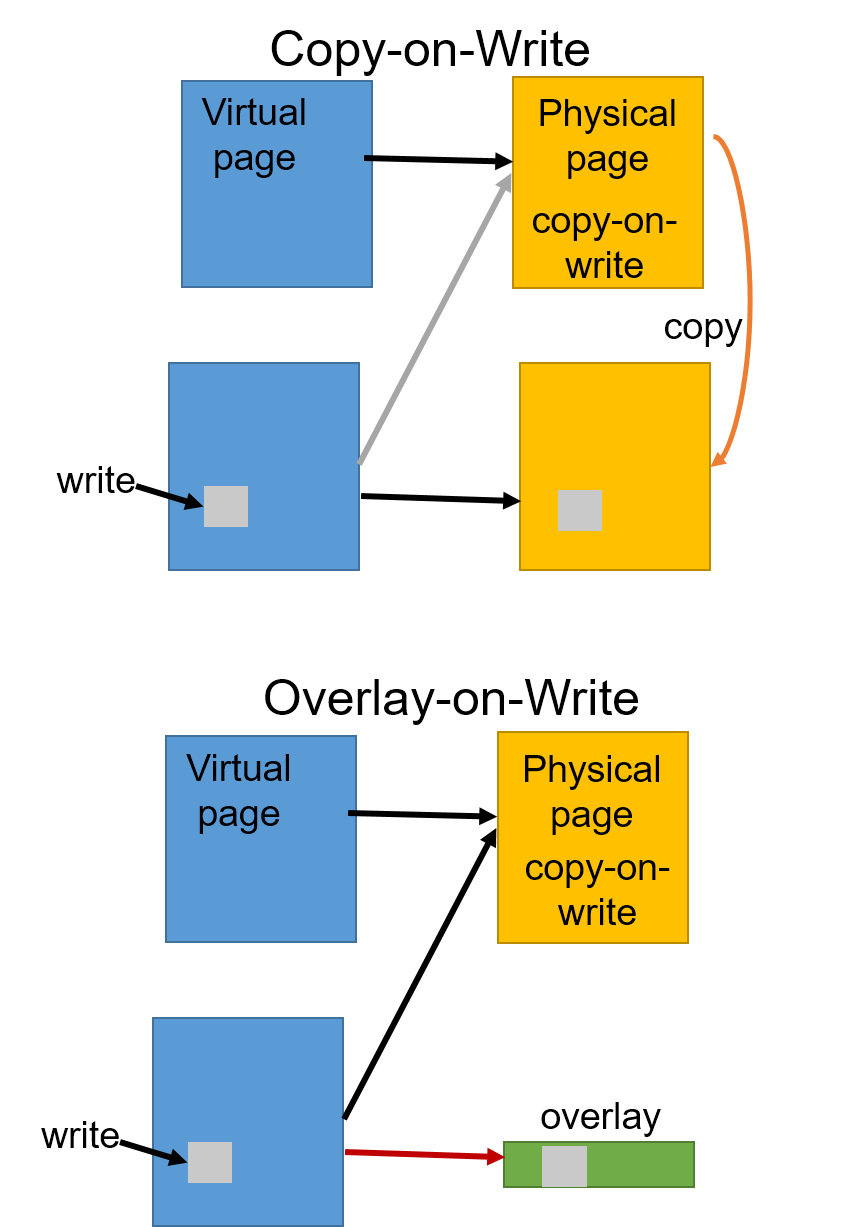
\includegraphics[width=2in]{Figures/Picture2}
    \caption{The difference between copy-on-write and overlay-on-write}
    \label{fig:oow}
\end{figure}


% !TEX root = ../Thesis.tex
\chapter{Evaluation}

We use the trap-driven simulation framework discussed in the previous chapter to simulate a system with superpage overlays. The workload we use for evaluation is a simulated memory checkpointing system with configurable properties.

For a simple motivational study, the fork-write benchmark is analyzed without simulation using the Linux \verb|perf| tool. Figure \ref{fig:tables} shows the average time and TLB misses for the different configurations of the benchmark, measured by the Linux perf tool. Either a superpage or 512 small pages are allocated, and either one small page or the entire 2MB region is written to in the child process. This benchmark demonstrates the potential for superpage overlays to improve performance. Writing to many 4KB pages is slow due to the high number of TLB misses, but doing copy-on-write with a superpage is slow compared to the 4KB pages when the writes only affect a small amount of memory. Superpage overlays should provide the TLB benefits of superpages while only copying 4KB at a time when the child process writes.
\begin{figure}
    \centering
    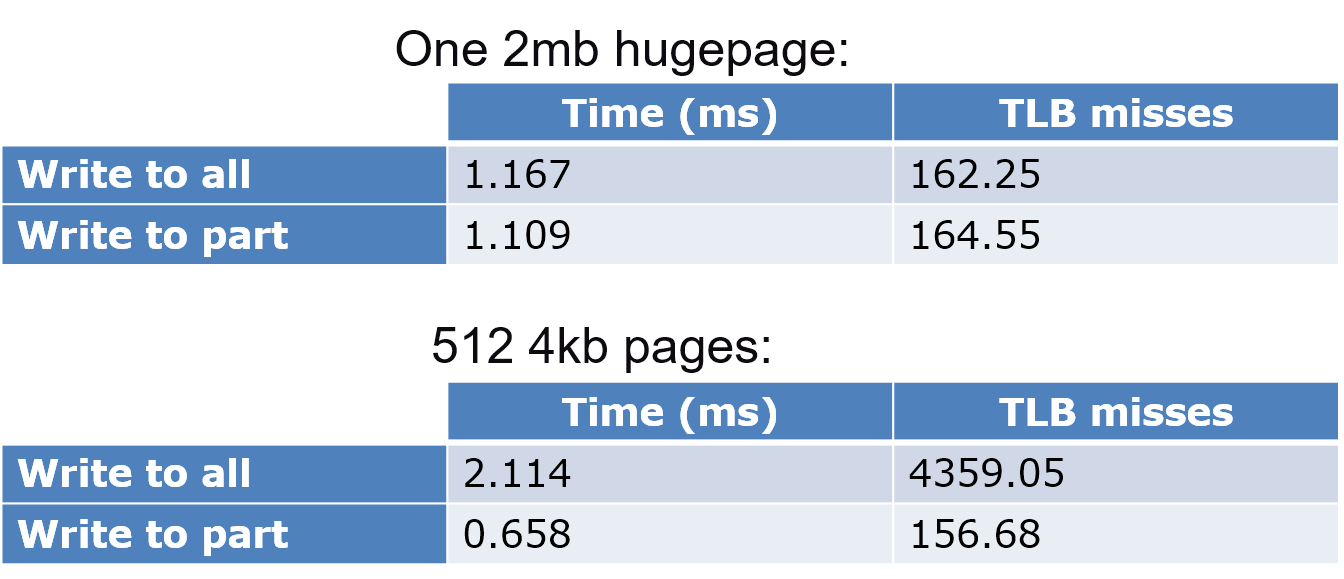
\includegraphics[width=3.2in]{Figures/Table1}
    \caption{Real TLB misses and elapsed time for the 4 different configurations of the fork-write benchmark}
    \label{fig:tables}
\end{figure}

\section{Using Trap-Driven Simulation}

Simulating superpage overlays in the trap-driven framework is fairly simple. We define a \verb|superpage_info| struct that tracks simulation data for every superpage. It includes the virtual and physical address, a flag that is set when the page is marked COW, and the OBitVector. The COW flag is used to identify when the overlay bit should be set for any write to the superpage. When a TLB miss causes a page fault, we can use the information from the page fault and these structs to determine wheter to send the address to the simulated 4KB or 2MB TLB for updating. There are 4 possibilities depending on whether the address is a small page or superpage in the real system and whether there is a \verb|superpage_info| struct.

\begin{enumerate}
\item small page fault, no \verb|superpage_info|:
\begin{itemize}
  \item 4KB TLB query
  \item check if superpage coalescing candidate and make \verb|superpage_info| if so
\end{itemize}

\item superpage fault, no \verb|superpage_info|:
\begin{itemize}
  \item 2MB TLB query
  \item create a \verb|superpage_info| and add it to the list
\end{itemize}

\item small page fault, found \verb|superpage_info|:
\begin{itemize}
  \item 2MB TLB query
  \item if physical address not aligned: set overlay bit
  \item if overlay bit set: 4KB TLB query
  \item check if overlay resetting is required and remove \verb|superpage_info| if so
\end{itemize}

\item superpage fault, found \verb|superpage_info|:
\begin{itemize}
  \item 2MB TLB query
  \item if overlay bit set: 4KB TLB query
\end{itemize}
\end{enumerate}

The 4KB and 2MB TLBs being queried are both regular caches with 128 entries and 4-way associativity by default, and the NRU eviction policy discussed in the Trap-Driven Simulation chapter. Every page that is evicted is cleared from the real TLB so that the next access that would miss in the simulated TLB will cause another page fault.

There is also a second simulated TLB that simply models the behavior of a normal system without superpage overlays. It is set up the exact same way, but none of the tests involving \verb|superpage_info| are done. Thus, the superpage overlay system can be compared to a system without overlays with a single benchmark run.

\section{Memory Checkpointing Simulation}

In the Design chapter two forms of memory checkpointing were discussed. Both can be simulated in the same way, since we need not worry about what actually happens to the checkpointed data for the purposes of evaluating superpage overlays. The only difference is that the first type incrementally marks pages writable again as the checkpoint is written out, while the second marks everything writable at once when a commit occurs. We use the first type for this evaluation, though the results would be essentially the same.

The simulation does everything that a real memory checkpointing framework would do, except that the memory snapshots are not actually saved anywhere or used in any way. All writable pages in the address space are marked read-only, and a kernel thread iterates through and waits a small amount of time per page to simulate writing it to nonvolatile memory before clearing the read-only flag and continuing. This checkpoint operationg runs once per second.

While the checkpoint is in progress, writes to the pages that are still read-only will be detected and a simulation of COW will occur. If the page is a superpage, there are three different types of COW operation that are compared in this evaluation:

\begin{enumerate}
  \item The superpage is simply copied in whole when a write occurs to any part of it. This is the default COW behavior of Linux.
  \item The superpage is split into small pages and only one 4KB page is copied.
  \item The 4KB segment of the superpage is copied into an overlay.
\end{enumerate}

It is clear that options 2 and 3 will copy the same amount of data. Option 1 will have the fewest TLB misses, since all the memory stays in superpages, while 2 will have the most because all the superpages will soon be split.

The simulation framework is also updated to track the overlays created due to checkpoints separately and implement overlay switching for those pages to limit the number of overlays that exist after many checkpoint iterations. In this way, repeated checkpointing effectively causes superpages to bounce back and forth between two physical memory locations.

\section{Checkpoint Workload}

The last component needed for evaluation is a userspace program to run the checkpoints on. This is just a simple benchmark that simulates a generic memory-intensive workload. The program allocates a large region of memory (which is allocated as superpages via THP), and repeatedly reads or writes random bytes of memory. The percentage of accesses that are writes is configurable, and there is also a locality parameter.

The locality sets the probability distribution of memory access locations. A higher locality means that each access is more likely to be near the previous one. This approximates the behavior of most programs, since in general accesses are likely to cluster around a ``hot'' region. The locality is implemented by setting the probability $p$ of stepping 4KB at a time up or down in memory. A direction is picked randomly, and the program loops, deciding on each iteration whether to take another step or stop based on $p$. Then a read or write is performed at the chosen location based on the write probability.

\section{Goals}

The overall goal of this evaluation is to demonstrate the advantages of using superpage overlays. Memory checkpointing is used as an easy-to-analyze example of a situation that is well suited to overlays, as well as a practical proposal for a tool that becomes much more useful when overlays are enabled. If overlays reduce the impact of checkpoints enough, it may become practical to implement frequent checkpointing in many applications to enable easy error recovery.

Additionally, the memory checkpointing application is a demonstration of the general usefulness of superpage overlays. Any application that heavily relies on COW will behave similarly and get the same benefits. Applications that frequently cause superpages to split will similarly benefit, since any operation that splits a superpage for finer-grained memory management could use overlays to avoid splitting and retain the benefits of superpages.


%\input{Chapters/Chapter4}

%\input{Chapters/Chapter5}

%\input{Chapters/Chapter6} % Results and Discussion

%\input{Chapters/Chapter7} % Conclusion

%% ----------------------------------------------------------------
% Now begin the Appendices, including them as separate files

\addtocontents{toc}{\vspace{2em}} % Add a gap in the Contents, for aesthetics

\appendix % Cue to tell LaTeX that the following 'chapters' are Appendices

%\chapter{An Appendix}

Lorem ipsum dolor sit amet, consectetur adipiscing elit. Vivamus at pulvinar nisi. Phasellus hendrerit, diam placerat interdum iaculis, mauris justo cursus risus, in viverra purus eros at ligula. Ut metus justo, consequat a tristique posuere, laoreet nec nibh. Etiam et scelerisque mauris. Phasellus vel massa magna. Ut non neque id tortor pharetra bibendum vitae sit amet nisi. Duis nec quam quam, sed euismod justo. Pellentesque eu tellus vitae ante tempus malesuada. Nunc accumsan, quam in congue consequat, lectus lectus dapibus erat, id aliquet urna neque at massa. Nulla facilisi. Morbi ullamcorper eleifend posuere. Donec libero leo, faucibus nec bibendum at, mattis et urna. Proin consectetur, nunc ut imperdiet lobortis, magna neque tincidunt lectus, id iaculis nisi justo id nibh. Pellentesque vel sem in erat vulputate faucibus molestie ut lorem.

Quisque tristique urna in lorem laoreet at laoreet quam congue. Donec dolor turpis, blandit non imperdiet aliquet, blandit et felis. In lorem nisi, pretium sit amet vestibulum sed, tempus et sem. Proin non ante turpis. Nulla imperdiet fringilla convallis. Vivamus vel bibendum nisl. Pellentesque justo lectus, molestie vel luctus sed, lobortis in libero. Nulla facilisi. Aliquam erat volutpat. Suspendisse vitae nunc nunc. Sed aliquet est suscipit sapien rhoncus non adipiscing nibh consequat. Aliquam metus urna, faucibus eu vulputate non, luctus eu justo.

Donec urna leo, vulputate vitae porta eu, vehicula blandit libero. Phasellus eget massa et leo condimentum mollis. Nullam molestie, justo at pellentesque vulputate, sapien velit ornare diam, nec gravida lacus augue non diam. Integer mattis lacus id libero ultrices sit amet mollis neque molestie. Integer ut leo eget mi volutpat congue. Vivamus sodales, turpis id venenatis placerat, tellus purus adipiscing magna, eu aliquam nibh dolor id nibh. Pellentesque habitant morbi tristique senectus et netus et malesuada fames ac turpis egestas. Sed cursus convallis quam nec vehicula. Sed vulputate neque eget odio fringilla ac sodales urna feugiat.

Phasellus nisi quam, volutpat non ullamcorper eget, congue fringilla leo. Cras et erat et nibh placerat commodo id ornare est. Nulla facilisi. Aenean pulvinar scelerisque eros eget interdum. Nunc pulvinar magna ut felis varius in hendrerit dolor accumsan. Nunc pellentesque magna quis magna bibendum non laoreet erat tincidunt. Nulla facilisi.

Duis eget massa sem, gravida interdum ipsum. Nulla nunc nisl, hendrerit sit amet commodo vel, varius id tellus. Lorem ipsum dolor sit amet, consectetur adipiscing elit. Nunc ac dolor est. Suspendisse ultrices tincidunt metus eget accumsan. Nullam facilisis, justo vitae convallis sollicitudin, eros augue malesuada metus, nec sagittis diam nibh ut sapien. Duis blandit lectus vitae lorem aliquam nec euismod nisi volutpat. Vestibulum ornare dictum tortor, at faucibus justo tempor non. Nulla facilisi. Cras non massa nunc, eget euismod purus. Nunc metus ipsum, euismod a consectetur vel, hendrerit nec nunc.	% Appendix Title

%\input{Appendices/AppendixB} % Appendix Title

%\input{Appendices/AppendixC} % Appendix Title

\addtocontents{toc}{\vspace{2em}}  % Add a gap in the Contents, for aesthetics
\backmatter

%% ----------------------------------------------------------------
\label{Bibliography}
\lhead{\emph{Bibliography}}  % Change the left side page header to "Bibliography"
\bibliographystyle{unsrtnat}  % Use the "unsrtnat" BibTeX style for formatting the Bibliography
\bibliography{Bibliography}  % The references (bibliography) information are stored in the file named "Bibliography.bib"

\end{document}  % The End
%% ----------------------------------------------------------------
